\chapter{Propuesta de calibración interna por acoplamientos mutuos}
\label{ch:mutualCalibration}
\lhead{\emph{Propuesta de calibración interna por acoplamientos mutuos}}

En este capítulo se presenta el método propuesto, calibración interna por acoplamientos mutuos, el cual complementa al método de
calibración interna clásico de manera tal que se pueda corregir, por ejemplo, la planitud del frente de onda emitido por la
antena. Primero, se explica en qué consiste y que recaudos hay que tomar a la hora de implementar este método de calibración.
Segundo, se expresa el modelo matemático y la cantidad de ecuaciones necesarias para encontrar una solución. Tercero, se
presentan tres posibles modos de ejecución y por último se exponen las limitaciones del método.  


\section{Descripción del método}

El método por acoplamientos mutuos toma ventaja del acoplamiento mutuo inherente y presente en toda la antena como la que se ha
presentado, entre los elementos radiantes. De hecho, cuando un ER transmite todos los demas reciben un aporte del mismo como así
también dicho elemento recibe el aporte de todos los ER que transmiten en simultáneo a él. La figura \ref{fig:mutualCoupling1}
muestra un ejemplo de lo anteriormente mencionado.

\begin{figure}[H]
 \centering
 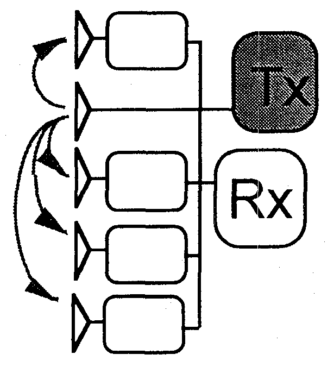
\includegraphics[width=4cm]{gfx/mutualCoupling1.png}
 \caption{Acoplamiento mutuo inherente de una antena \cite{Hara1997}.}
 \label{fig:mutualCoupling1}
\end{figure}

Para llevar a cabo dicho método, este tipo de antenas debe cumplir un requerimiento muy importante que es poder transmitir con
un elemento radiante y simultáneamente recibir con otro sin que se sature, de forma tal de trabajar en la zona lineal, o peor
aún, que se dañe o destruya. Normalmente, este requerimiento implica separar las redes de transmisión y recepción
\cite{Gao2001}. Para antenas que no cumplen la separación de las redes de transmisión y recepción aún se puede utilizar esta
idea si se transmite en una polarización y se recibe en otra, pues son dos lineas físicamente separadas.

Se tienen una serie de requisitos básicos para poder implementar este método que deben ser tenidos en cuenta desde el diseño
mismo.

\begin{enumerate}
	\item Modos de TRMs: Cada TRM debe tener tres modos de funcionamiento posibles, los cuales son Tx, Rx y protegido.
	\item Control Individual de TRMs: Se debe poder comandar desde la UCC el estado o modo individual de cada TRM, de esta forma, 
		se puede determinar que TRM estará en transmisión, en recepción y en modo protegido.
	\item Acoplamiento cruzado: Dado que la potencia de transmisión generalmente es mayor que la máxima posible en recepción, se
		debe utilizar la polarización cruzada para recibir dado que posee una mayor aislación, si se transmite por H se debe recibir
		por V y viceversa.
	\item Seguridad: Se debe incorporar al menos una línea física de control de estado de TRMs redundante con el objetivo de
		minimizar el riesgo de daño por acoplamiento mutuo. Por ejemplo, al de tener dos ER cercanos transmitiendo y recibiendo en
		simultáneo por la rotura de una línea de control.
\end{enumerate}


\subsection{Establecimiento de zonas de acoplamiento mutuo} \label{ssc:mutual_zone}

Dado que las antenas poseen una potencia de recepción máxima, límite donde los componentes pueden resultar dañados, y dado
que el acoplamiento mutuo depende de la distancia y de la aislación entre polarizaciones cruzadas, el método no es aplicable a
cualquier par de elementos radiantes.

En general, se pueden establecer tres zonas, que dependen de la distancia al elemento que está en transmisión. Estas zonas se
llaman de acoplamiento destructivo, lineal y de acoplamiento débil. El método solamente es aplicable en la zona lineal.
Asumiendo que el nivel de potencia con el que se transmite desde el elemento central es único y fijo, la figura \ref{fig:levels}
ejemplifica las tres zonas de recepción al emitir con el elemento radiante central:
\begin{itemize}
	\item En gris oscuro: zona de acoplamiento destructivo. Los TRMs deben estar en modo protegido o alta impedancia, en este modo
		no se transmite ni se recibe señal.
	\item En gris: zona de acoplamiento lineal. La potencia está dentro de los límites aceptables para aplicar el método.
	\item En gris claro: zona de acoplamiento débil. No se puede aplicar el método dado que el nivel de señal es inferior al piso
		de ruido. 
\end{itemize}

\begin{figure}[H]
 \centering
 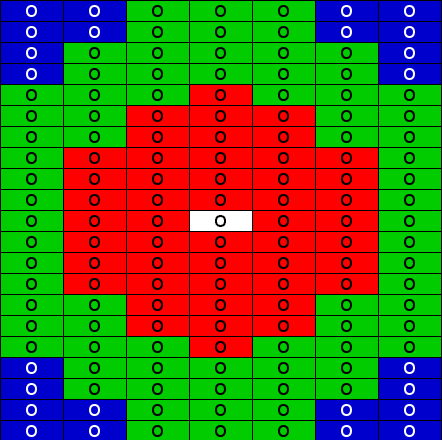
\includegraphics[width=9cm]{gfx/mutualCouplingLevels.png}
 \caption{Zonas de acoplamientos de la antena al emitir con el ER central. En gris oscuro, acoplamiento destructivo; en gris,
 acoplamiento lineal y en gris claro acoplamiento débil.}
 \label{fig:levels}
\end{figure}

Tomando en cuenta lo anteriormente mencionado, determinando la potencia de transmisión y considerando que el acoplamiento mutuo
depende de la distancia entre ER y el rango de potencia en recepción admisible, se pueden determinar todos los posibles lazos de
calibración del método.


\subsection{Control de estados de TRMs}

Como cada TRM puede estar en uno de sus tres estados posibles, Tx, Rx o protegido, se debe determinar de que forma la UCC
controla dichos estados. Una vez elegidos los ER que conforman el lazo de calibración, se establecen en modo protegido todos
aquellos TRMs que pertenecen a la zona de acoplamiento destructivo. A su vez, para evitar que el resto de los elementos que no
conforman parte del lazo activo de calibración interfieran, inyectando ruido en las redes de transmisión y/o recepción, se los
debe configurar en modo protegido. 

En la figura \ref{fig:mutual_general} se puede observar un ejemplo donde el lazo de calibración es determinado por la línea
gris, el TRM de polarización H conectado al elemento radiante $e_1$ está configurado en modo transmisión, el TRM en
polarización V conectado a $e_0$ está configurado en modo recepción y el resto están en modo protegido. Se asume que el
acoplamiento mutuo de dicho lazo de calibración pertenece a la zona de acoplamiento lineal.
\begin{figure}[H]
 \centering
 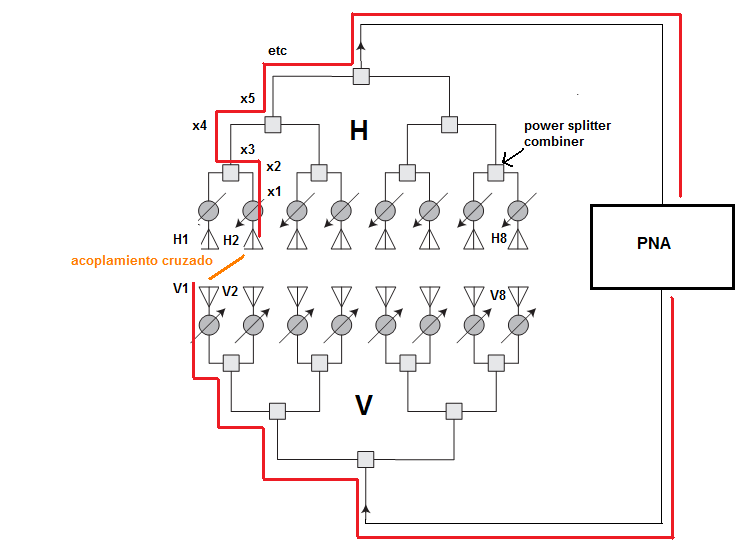
\includegraphics[width=9cm]{gfx/mutualCouplingExample.png}
 \caption{Ejemplo de calibración utilizando acoplamientos mutuos, transmitiendo en polarización H y recibiendo en V}
 \label{fig:mutual_general}
\end{figure}


\subsection{Análisis de factibilidad} \label{ssc:feasibility}

Como el método de calibración debe obtener tanto la potencia y fase de la antena transmitida y recibida como la planitud de
la misma, se deben determinar la cantidad de incógnitas y la cantidad de lazos de calibración, que implican el número de 
ecuaciones.

Si se modifican secuencialmente todos los receptores y luego todos los emisores del lazo de calibración de la figura
\ref{fig:mutual_general}, asumiendo que todos los acoplamientos mutuos pertenecen a la zona de acoplamiento lineal, se pueden obtener 
todos los lazos de calibración posibles para la polarización de transmisión H y recepción en V. Si se repite el proceso
cambiando las polarizaciones de transmisión y recepción se logran obtener todos los lazos posibles.

Asumiendo un conjunto de antena polarimétrica con una configuración de $M$ por $N$ elementos radiantes, que todos los
acoplamientos pertenecen a la zona lineal y que se transmite y recibe de a un ER por lazo, se disponen de $(M\cdot N)^2$ lazos
por polarización a transmitir. Totalizando en $2(M\cdot N)^2$.

Para determinar la cantidad de incógnitas es importante destacar que el receptor de la UCC mide tanto fase como potencia de la
señal, de esta forma, se utilizarán valores complejos tanto para las señales medidas por la UCC, como para las incógnitas.

Asumiendo el mismo conjunto de antena polarimétrica de $M$ por $N$ elementos radiantes, como se puede transmitir y recibir en
dos polarizaciones (H y V), la antena cuenta con $4M\cdot N$ incógnitas de potencia de señal transmitida/recibida (2 por Tx en H/V y
otras 2 por Rx en H/V).

En el apéndice \ref{AppendixA} se realiza el cálculo de la cantidad de acoplamientos mutuos que posee un conjunto de antena
polarimétrica, particularmente, la ecuación \ref{eq:amountMutCoupling} muestra la cantidad de incógnitas, que, para este caso,
resulta ser de $M\cdot N(M\cdot N-1)/2$. Por lo tanto, este conjunto de antena posee en total $M\cdot N(M\cdot N + 7)/2$ incógnitas.

Para obtener el menor conjunto de antena al cual el método es aplicable, la cantidad de lazos, que determina la cantidad de
ecuaciones, debe ser mayor a la cantidad de incógnitas, 
$$
\begin{aligned}
	2(M\cdot N)^2 &\ge  \dfrac{M\cdot N(M\cdot N + 7)}{2} \\
	4M\cdot N &- M\cdot N \ge7 \\
	M\cdot N &\ge \dfrac{7}{3}
\end{aligned}
$$

Como $M$ y $N$ son números enteros, la cantidad mínima de elementos radiantes que puede tener un conjunto de antena, asumiendo
que todos los acoplamientos mutuos pertenecen a la zona lineal, es tres.

La herramienta matemática utilizada para resolver el sistema de ecuaciones es el de los cuadrados mínimos,
ver apéndice \ref{AppendixB}, con el cual se obtiene la aproximación que tenga menor error cuadrático medio.


\subsection{Modos de operación}
\label{ssc:operationalModes}

En esta sección se presentarán tres modalidades de este método, las diferencias entre dichas modalidades es la de si se asumen
conocidos los acoplamientos mutuos. Dado que las variaciones mecánicas son lentas con respecto a las variaciones eléctricas
(por ejemplo inestabilidades en temperatura o de tensión), si se realizan calibraciones lo suficientemente seguidas se pueden
llegar a reutilizar los resultados obtenidos de los acoplamientos mutuos para disminuir la cantidad de incógnitas, por lo tanto
la cantidad de ecuaciones necesarias, o lazos de calibración. Los diferentes modos de operación se listan a continuación:

\begin{itemize}
	\item \textbf{Modo completo:} En esta modalidad se estima la ganancia en transmisión y en recepción, respectivamente, en ambas
		polarizaciones H y V. Se determinan ademas los valores de acoplamientos mutuos. La cantidad de ecuaciones necesarias es de
		$M\cdot N(M\cdot N + 7)/2$, ver sección \ref{ssc:feasibility}.
	\item \textbf{Modo parcial:} En esta modalidad se estima la ganancia en transmisión y recepción, respectivamente, en ambas
		polarizaciones H y V reutilizando el valor guardado de la planitud de la antena calculado previamente. La cantidad de
		ecuaciones necesarias es de $4M\cdot N$, ver sección \ref{ssc:feasibility}.
	\item \textbf{Modo planitud ideal:} Esta modalidad, la cual es la desarrollada en la tesis, posee la misma cantidad de
		ecuaciones que el modo rápido, la diferencia es que se asume que la antena es perfectamente plana.
\end{itemize}


\subsection{Método}

Asumiendo que se transmite desde el elemento radiante $m$, denotado como $e_m$, y se recibe desde el elemento radiante $n$,
denotado como $e_n$, la función de transferencia del lazo de calibración de los elementos participantes $L_{m,n}$ está
compuesta por:

\begin{enumerate}
	\item La configuración de atenuación y desfase de los atenuadores y desfasadores, tanto de transmisión como de recepción,
		denotados como $w_{Tm}(i)$ y $w_{Rn}(j)$ respectivamente, donde $i$, $j$ son las diferentes posibles configuraciones.
	\item La atenuación y desfase combinados por los cables, conectores, divisores y combinadores de potencia, módulos radiantes
		y desfasadores de transmisión y recepción, denotados como $u_{Tm}$ y $u_{Rn}$ respectivamente.
	\item El acoplamiento mutuo entre los elementos participantes, denotado como $C_{m, n}$.
\end{enumerate}

Por lo tanto, la función de transferencia completa resulta,

\begin{equation}
	L_{m,n} = w_{Tm} \cdot u_{Tm} \cdot C_{m,n} \cdot w_{Rn} \cdot u_{Rn}
	\label{eq:transfer_mn}
\end{equation}
donde el primer elemento del subíndice de $L$ es el transmisor y el segundo el receptor. Si se transmite con el mismo elemento,
$e_m$, pero se recibe con otro, $e_{n + 1}$, la transferencia resulta

\begin{equation}
	L_{m,n + 1} = w_{Tm} \cdot u_{Tm} \cdot C_{m,n + 1} \cdot w_{Rn + 1} \cdot u_{Rn + 1}
	\label{eq:transfer_mn1}
\end{equation}

Tomando la relación de ambas transferencias \ref{eq:transfer_mn} y \ref{eq:transfer_mn1}, 

\begin{equation}
	W^{m}_{Rn,n + 1} = \dfrac{L_{m,n}}{L_{m,n + 1}} = \dfrac{C_{m,n} \cdot w_{Rn} \cdot u_{Rn}}{C_{m,n + 1} \cdot w_{Rn + 1} \cdot u_{Rn + 1}}
\end{equation}
donde el superíndice de la relación $W$ indica el elemento en común y el subíndice indica los otros elementos participantes y
sus modos, T para transmisión y R para recepción. El orden de los elementos del subíndice indican la relación, el primero va
en el numerador y el segundo en el denominador. Por ejemplo, en este caso en particular, se transmite por el elemento $m$ y
se recibe por los elementos $n$ y $n+1$, y la relación es de $\frac{L_{m,n}}{L_{m,n + 1}}$.

Se asume que el valor del acoplamiento depende de dos factores a saber. El primero es por comunicar los elementos utilizando
polarizaciones cruzadas, y dicha atenuación es constante para cualquier elemento. El segundo, es debido a la atenuación y
desfase de la señal que viaja en el vacío, por lo tanto, depende exclusivamente de la distancia que hay entre los elementos
a comunicar.

Ahora, si se combinan las funciones de transferencia $L_{m,n+1}$ y $L_{m,n+2}$, la relación resulta,

\begin{equation}
	W^{m}_{Rn + 1,n + 2} = \dfrac{L_{m,n+1}}{L_{m,n+2}} = \dfrac{C_{m,n+1} \cdot w_{Rn+1} \cdot u_{Rn+1}}{C_{m,n + 2} \cdot w_{Rn + 2} \cdot u_{Rn + 2}}
\end{equation}

Y si se combinan las funciones de transferencia $L_{m,n}$ y $L_{m,n+2}$,

\begin{equation}
	W^{m}_{Rn,n + 2} = \dfrac{L_{m,n}}{L_{m,n + 2}}\cdot\dfrac{L_{m,n+1}}{L_{m,n+1}} = W^{m}_{Rn,n+1}\cdot W^{m}_{Rn+1,n + 2}
\end{equation}


Generalizando, se pueden obtener todos los lazos de calibración en función de uno,

\begin{equation}
	W^{m}_{R0,k} = \prod_{i=0}^{k-1} W^{m}_{Ri,i+1} = \prod_{i=0}^{k-1}\dfrac{L_{m,i}}{L_{m,i+1}} =
		\prod_{i=0}^{k-1}\dfrac{C_{m,i} \cdot w_{Ri} \cdot u_{Ri}}{C_{m,i + 1} \cdot w_{Ri + 1} \cdot u_{Ri + 1}}
	\label{eq:rx_cal}
\end{equation}

Si se realiza la misma deducción, pero en vez de transmitir siempre con el mismo elemento, se lo utiliza para recibir, se obtiene

\begin{equation}
	W^{m}_{T0,k} = \prod_{i=0}^{k-1} W^{m}_{Ti,i+1} = \prod_{i=0}^{k-1}\dfrac{L_{i,m}}{L_{i+1, m}} =
		\prod_{i=0}^{k-1}\dfrac{w_{Ti} \cdot u_{Ti} \cdot C_{i,m}}{w_{Ti + 1} \cdot u_{Ti + 1} \cdot C_{i + 1, m}}
	\label{eq:tx_cal}
\end{equation}

Analizando las ecuaciones \ref{eq:rx_cal} y \ref{eq:tx_cal}, surgen las primeras dos conclusiones. La primera es que el
resultado no es único, por lo tanto, en principio, con este método no se pueden obtener ganancias absolutas (de transmisión,
recepción y acoplamientos mutuos), solamente ganancias relativa entre dichos elementos. La segunda, es que el sistema tiene
dos grados de libertad, en otras palabras, para poder obtener las ganancias absolutas de transmisión, recepción y acoplamientos
mutuos, es necesario agregar dos ecuaciones más que definan algún valor perteneciente a dos de los tres conjuntos de incógnitas.

Al asumir que a misma distancia el acoplamiento mutuo es el mismo o si se los reutilizan de una calibración anterior, las
ecuaciones \ref{eq:rx_cal} y \ref{eq:tx_cal} se simplifican, logrando que la cantidad de incógnitas se reduzca habilitando
de esta forma el método de planitud ideal y el parcial respectivamente.

Como es necesaria una menor cantidad de ecuaciones de calibración, se opta por una estrategia de lazos simétricos con un
elemento en común. Al restar ambos caminos, no solo se elimina la RFDN común, sino que también se elimina el
acoplamiento mutuo. La cantidad de estos lazos termina siendo determinada como una solución de compromiso entre la cantidad 
mínima necesaria para poder utilizar el método y la cantidad de ecuaciones redundantes para disminuir la incertidumbre en el
resultado. Las ecuaciones para recepción y transmisión simplificadas resultan.

\begin{equation}
	W^{'}_{R0,k} = \prod_{i=0}^{k-1} W^{'}_{Ri,i+1} = \prod_{i=0}^{k-1}\dfrac{w_{Ri} \cdot u_{Ri}}{w_{Ri + 1} \cdot u_{Ri + 1}} =
	\dfrac{w_{R0} \cdot u_{R0}}{w_{Rk} \cdot u_{Rk}}
	\label{eq:rx_simp_cal}
\end{equation}

\begin{equation}
	W^{'}_{T0,k} = \prod_{i=0}^{k-1} W^{'}_{Ti,i+1} = \prod_{i=0}^{k-1}\dfrac{w_{Ti} \cdot u_{Ti}}{w_{Ti + 1} \cdot u_{Ti + 1}} =
	\dfrac{w_{T0} \cdot u_{T0}}{w_{Tk} \cdot u_{Tk}}
	\label{eq:tx_simp_cal}
\end{equation}

Si el RM común se utiliza para transmitir la señal, se obtienen ecuaciones para calibrar la parte de recepción, en cambio,
si se lo utiliza para recibir la señal, se calibra transmisión. La figura \ref{fig:ideal_strategy} esquematiza esta estrategia.

\begin{figure}[H]
 \centering
	\subfloat[]{
		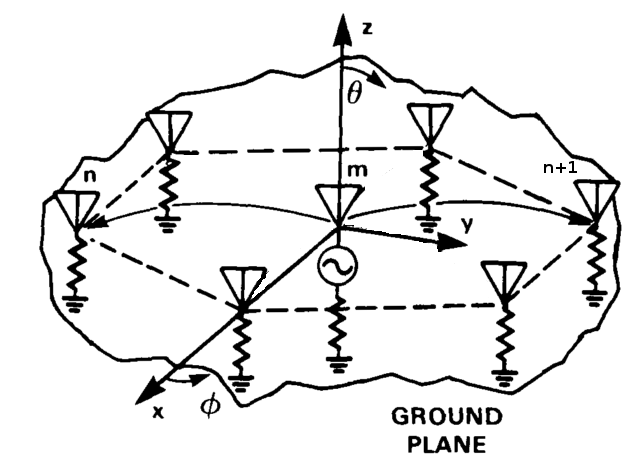
\includegraphics[width=6cm]{gfx/mutualRxCal.png}}
	\subfloat[]{
		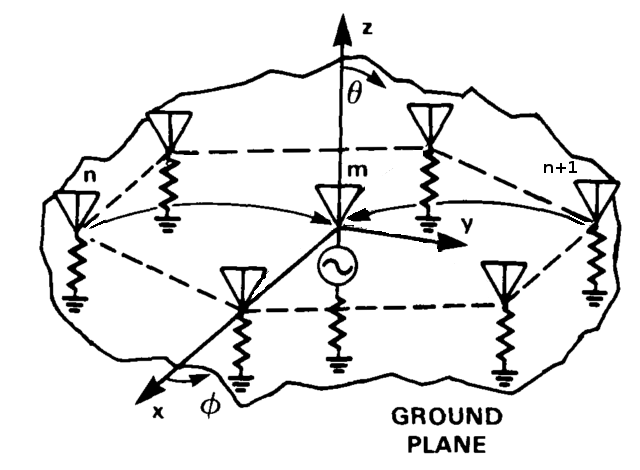
\includegraphics[width=6cm]{gfx/mutualTxCal.png}}
	\caption{estrategia de planitud ideal. (a) Calibra lazos de recepción, (b) Calibra lazos de transmisión \cite{Aumann1989}.}
 \label{fig:ideal_strategy}
\end{figure}


\subsection{Determinación de la fase} \label{ssc:mutualPhase}

Como el método de resolución utilizado en este método es de naturaleza lineal, resolviendo ecuaciones de la siguiente forma
$Ax = b$, y como la fase de una señal es de naturaleza modular, de 360 grados, se pueden cometer errores en la resolución.
Dependiendo de cómo sea $A$ y qué valores tenga $x$, $b$ no necesariamente está contenido dentro del conjunto solución (en
módulo 360) generando así un error en la resolución de la estimación del valor $x$.

Para ejemplificar, se asume que se tiene un conjunto de antena de tres elementos radiantes. La RFDN (en Tx y Rx) desfasa 100
grados, el desfasador del primer elemento está configurado en 240 grados y el del tercero en 120, el acoplamiento mutuo no desfasa
y se utiliza la ecuación $\dfrac{L_{1,2}}{L_{3, 2}}$. La figura \ref{fig:phaseDetermination} muestra la antena con los 
lazos de calibración utilizados.

\begin{figure}[H]
 \centering
 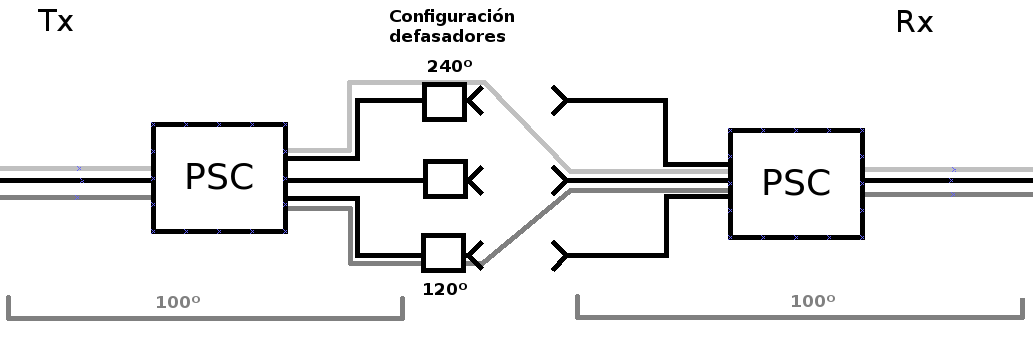
\includegraphics[width=10cm]{gfx/loopCal.png}
 \caption{Lazo de calibración de una antena polarimétrica}
 \label{fig:phaseDetermination}
\end{figure}

Utilizando la ecuación previamente mencionada, $A$ resulta ser
$$
	\mathbf{A} = \begin{pmatrix} 1 & 0 & -1\end{pmatrix}
$$

El verdadero valor de x resulta ser la contribución de la rama de transmisión junto a la configuración del desfasador del TRM,
$$
	\mathbf{x} = \begin{pmatrix} 340 \\ x \\ 220\end{pmatrix}
$$

Al resolver la ecuación $Ax$ se obtiene el resultado de 120 grados. Si la fase fuese de naturaleza lineal, este sería el valor 
resultante de la resta de la medición de ambos lazos de calibración. Las mediciones de dichos lazos resultan: 
\begin{itemize}
	\item La fase de $L_{1,2}$ es 440 grados, en módulo 360 resulta igual a 80 grados (100 grados por la rama de
		transmisión sumado a 240 por el desfasador del primer TRM y 100 grados más por la rama de recepción).
	\item La fase de $L_{3, 2}$ es 320 grados (100 grados por la rama de transmisión sumado a 240 por el desfasador
		del primer TRM y 100 grados más por la rama de recepción).
\end{itemize}

La resta de dichas mediciones deberían ser igual a 120 grados, pero se observa que es igual a -240 grados generando así un
error en la estimación de la fase.

Para solucionar esto, la estrategia propuesta es la de reutilizar el valor estimado de $x$ de una calibración previa, calcular
el $b$ ideal y modificar los valores de $b$ de la calibración actual sumando o restando de a 360 grados para acercarse lo más 
posible a dichos valores esperados. Para la primera calibración, es necesario medir cuanto desfasa la antena en al menos una 
rama punta a punta. 


\subsection{Limitaciones}

Si bien este método de calibración interna por acoplamientos mútuos abarca completamente la antena posibilitando determinar las
ganancias de transmisión, recepción y la planitud de la antena, presenta las siguientes limitaciones.


\subsubsection{Determinación de ganancia y fase absoluta}

Dado que todas las ecuaciones del método son de relaciones entre caminos de calibración, no se puede determinar la potencia y
fase absoluta transmitida o recibida. Para poder obtener dichos valores es necesario agregar dos ecuaciones extra.

Una posible estrategia es la de utilizar el resultado obtenido al correr el método de calibración interna clásica obteniendo
así la ganancia y fase de uno de los caminos de transmisión y recepción. Otra posibilidad es la de utilizar dos antenas
dedicadas y bien caracterizadas para ser utilizadas en modo transmisión y recepción para la calibración.


\subsubsection{Comportamiento modular de la fase medida}

Dado que el método de calibración por acoplamientos mutuos es de carácter lineal y la fase es de carácter modular, es necesario 
conocer el orden del valor del desfase de los caminos de Tx y Rx punta a punta. Utilizando dichos valores como entrada en la
calibración se evitan los posibles errores de cálculos al obtener la fase de transmisión y recepción de la antena, ver
\ref{ssc:mutualPhase}. Dichos valores solo serán utilizados una vez, dado que las subsiguientes calibraciones reutilizarán los
valores de fase obtenidos de la calibración anterior.

Para obtener dicho valor inicial, se puede utilizar la fase resultante del método de calibración interna clásica o se puede
realizar una medición de campo cercano en temperatura, emitiendo sólamente con un elemento radiante para deducir la fase de la
red de transmisión. Para obtener el desfase de la red de recepción, se emite con un elemento externo y se recibe con solo un
elemento radiante.


\subsubsection{Zona de acoplmaiento mutuo destructivo y bajo acoplamiento}

Generalmente, esta clase de antena transmite en una potencia mayor a la admisible en recepción, por lo tanto, los ERs cercanos al
de transmisión pueden resultar dañados si no se los coloca en un estado protegido, evitando así que dicho par de elementos
radiantes, de transmisión y recepción, sean utilizados en un lazo de calibración.

Los ERs lejanos al de transmisión pueden llegar a recibir la señal de calibración con potencia menor al piso de ruido (zona de
acoplamiento débil), evitando también que dichos lazos de calibración sean útiles.

Para determinar las zonas de acoplamientos mutuos, definidas en la sección \ref{ssc:mutual_zone}, es necesario realizar en tierra
una medición de acoplamientos mutuos del conjunto de antena.

\section{Conclusiones}

En este capítulo se presentó el método de calibración por acoplamientos mutuos. Su mayor ventaja es que abarca todo el sistema de
transmisión y recepción de la antena, logrando así poder determinar la potencia de transmisión, de recepción y la planitud de la
misma.

Otras ventajas de este método son que se pueden evitar costosas campañas de caracterización, dado que para su utilización no es
necesario agregar HW extra que haga mas complejo el diseño de la antena y que al haber superposición de caminos en los lazos de
calibración se disminuye la incertidumbre del resultado de las ganancias obtenidas.

Como desventaja, se debe tener extremo cuidado al determinar los lazos de calibración porque se pueden llegar a dañar TRMs si el
acoplamiento mutuo de los elementos radiantes del lazo pertenece a la zona de acoplamiento destructivo.

